\chapter{Software pro zařízení}

Tato kapitola se věnuje návrhu a vývoji software pro výsledné zařízení včetně zpracování přijatých dat na serveru a jejich zobrazení uživateli v grafické podobě. Jako první jsou rozebrány možnosti zpracovávání dat a na základě výběru vhodných služeb pro tyto účely je navržen obslužný firmware mikrokontroleru a další součásti zpracování dat.

\section{Server pro zpracování naměřených dat}

Důležitým rozhodnutím pro realizaci celého zařízení je vhodný výběr aplikací a služeb, ve kterých se budou naměřená data uchovávat a následně zpracovávat či zobrazovat. Na trhu existuje několik veřejně dostupných serverů, které umožňují přijímání dat skrze různé protokoly a jejich následné uchovávání a zpracovávání.

Mezi nejznámější služby patří ThingSpeak\footnote{\url{https://thingspeak.com/}}, který umožňuje integraci MATLAB skriptů které se spouštějí nad uloženými přijatými daty. Při využívání neplacené verze této služby jsme limitování maximálním počtem přijatých zpráv za den (\SI{8200}{}), maximální dobou běhu skriptů \SI{20}{\second} nebo třeba pouze čtyřmi neveřejnými kanály na jeden účet. Další nevýhodou je možnost přijímat do jednoho kanálu maximálně 8 proměnných, pokud bychom chtěli vizualizovat více dat, musíme je rozdělit do více kanálů a můžeme tak brzy narazit na limity účtu poskytovaného zdarma.

Dalším z možných serverů na příjem a zpracování dat je ubidots\footnote{\url{https://ubidots.com/}}. I tento server poskytuje licenci zdarma, která je určena pro nekomerční použití studenty a kutily, kteří si chtějí platformu vyzkoušet. Nachází se zde omezení například v počtu maximálně tří připojených zařízení a uchovávání dat po dobu maximálně jednoho měsíce. Každé připojené zařízení může zasílat ke zpracování maximálně \SI{10}{} měřených veličin.

Jednou z možností je využít Arduino Cloud\footnote{\url{https://docs.arduino.cc/cloud/iot-cloud}} od stejnojmenné společnosti Arduino. Jejich cloud nabízí také plán pro používání bez poplatků, zde se dostáváme na mnohem větší restrikce než u dříve zmíněných služeb. Připojena mohou být pouze dvě zařízení, zařízení musí být naprogramováno v jejich prostředí, jelikož není k dispozici API pro připojení jiných zařízení. Největší nevýhodou je uchovávání naměřených dat pouze jeden den, což je pro statistiky či sledování nepoužitelné.

Další z mnoha možností, jak uchovávat a zpracovávt naměřená data je vytvoření vlastního prostředí pro tyto účely. Lze použít spojení databázové aplikace, která bude uchovávat data (např. InfluxDB\footnote{\url{https://www.influxdata.com/}}) a dalších služeb pro příjem, zpracování a zobrazení těchto dat. Pro příjem zpráv od zařízení bude připojen Eclipse Mosquitto\footnote{\url{https://mosquitto.org/}}, což je tzv. MQTT broker, který je potřebný k přijímání dat zasílaných skrze protokol MQTT. Tento broker lze poté připojit přes Node-RED\footnote{\url{https://nodered.org/}}, což je programovací nástroj určený k jednoduchému propojení zařízení s dalšími službami, lze jej tedy použít pro zpracování přijatých zpráv a jejich následné uložení do databáze. Statistiky a přehledy lze vykreslovat pomocí služby Grafana\footnote{\url{https://grafana.com/}}. Všechny tyto nástroje jsou open-source a lze je využívat zdarma i pro komerční použití.

\section{Základní funkce zařízení}

Na obrázku \ref{fig_flowchart} je vidět základní koncept běhu programu pro mikrokontroler. Jedná se o jednoduchý stavový automat, který zajistí vykonání příkazů ve správném pořadí a zajišťuje čekání na přijmutí dat ze všech senzorů. V tomto zařízení jsou totiž využity senzory, které neposkytují změřená data okamžitě, ale až po delším časovém úseku svého provozu. Například senzor SGP30 pro měření TVOC a koncentrace CO$_2$ vrací prvních \SI{15}{\second} fixní hodnotu 400~ppm a až po uplynutí tohoto času začne vracet reálná naměřená data. Velice podobně pracuje i senzor koncentrace prachových částic, kde potřebuje být v provozu alespoň \SI{20}{\second} aby dokázal vrátit naměřená data.

\begin{figure}[h]
    \centering
    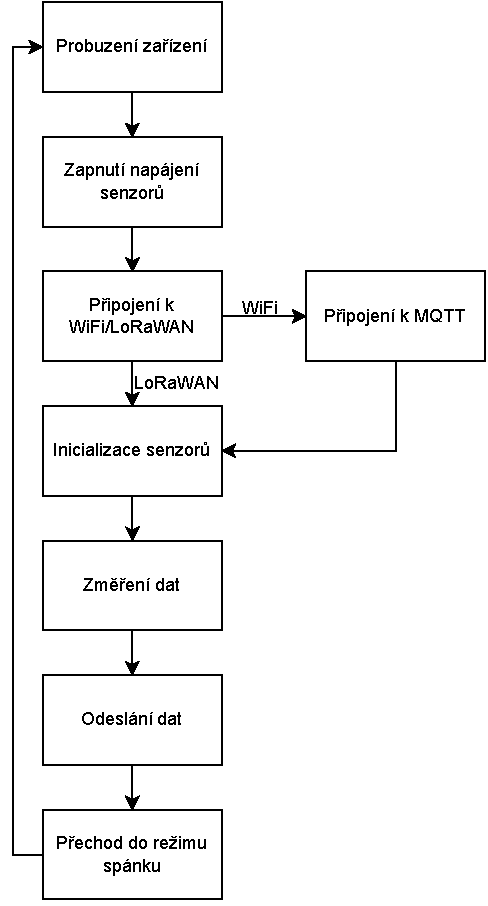
\includegraphics[width=0.4\textwidth]{obrazky/flowchart.pdf}
    \caption{Základní funkce softwaru pro mikrokontroler.}
    \label{fig_flowchart}
\end{figure}

Jak již bylo zmíněno v předchozích kapitolách, zařízení bude moci zasílat naměřená data pomocí WiFi nebo pomocí LoRaWAN sítě. Obě dvě sítě vyžadují projít procesem připojení, kde u WiFi zařízení dostane přidělenou IP adresu a u LoRaWAN dojde k vygenerování klíčů, pomocí kterých se poté šifrují a zasílají zprávy. Zařízení je koncipováno tak, že může být připojeno pouze k jedné z těchto sítí a toto nastavení je definováno pevně ve firmwaru zařízení. 

\section{Firmware mikrokontroleru}

Celý obslužný firmware pro mikrokontroler je naprogamován za použití frameworku ESP-IDF\footnote{\url{https://docs.espressif.com/projects/esp-idf/en/latest/esp32/}} přímo do výrobce čipu ESP32 Espressif. Tento framework obsahuje spousty knihoven pro obsluhu všech periferií a sběrnic, které čip obsahuje. Programování probíhá buďto v jazyce C nebo C\texttt{++}. Bylo zapotřebí napsat veškeré knihovny pro obsluhu připojených senzorů, tyto knihovny využívají již zmíněné knihovny od výrobce např. pro obsluhu sběrnice I$^2$C, SPI nebo UART.

Tento framework je postaven na projektu realtime operačního systému pro mikrokontrolery FreeRTOS\footnote{\url{https://www.freertos.org/}} a umožňuje tak jednoduše spouštět více vláken, časovače, spravovat fronty a uživatel se o to nemusí starat. Díky tomuto systému je software rozdělen do několika oddělených vláken, kde se starají o inicializaci WiFi rozhraní, spojení s MQTT brokerem, spojení a obsluhu LoRaWAN sítě, obsluhu senzorů na sběrnici I$^2$C, SPI nebo UART. Díky tomuto rozdělení do jednotlivých vláken je velice snadné zajistit správné časování pro jednotlivé čtení ze senzorů a je také možné používat blokující funkce pro čekání, jelikož blokováním jednoho vlákna nedojde k ovlivnění časování vlákna jiného.

\subsection{Obsluha senzorů}

Jak již bylo zmíněno, pro obsluhu všech připojených senzorů jsou použity vlastní knihovny založené na frameworku ESP-IDF. Tyto knihovny obsahují pouze potřebné čtení, inicializace a případné restarty senzorů. Není obsažena plná funkčnost dle datasheetu výrobce, jelikož pro tuto aplikaci nejsou všechny funkce senzorů potřebné. Senzory jsou rozděleny do skupin podle druhu použité komunikační sběrnice a je možné je jednotlivě softwarově vypínat, aby byla minimalizována spotřeba celého zařízení. Dále jsou také zajištěny již dříve zmíněné opakované vyčítání ze senzorů pro koncentraci CO$_2$ a senzoru prachových částic. Po ukončení jednotlivých měření jsou naměřená data uložena do datové struktury k pozdějšímu odeslání na server.

\subsection{Připojení k WiFi}

Pro použití zařízení s WiFi sítí je zapotřebí nakonfigurovat ve zdrojovém kódu použití této sítě a také další potřebné parametry. Konfigurace probíhá v souboru CMakeLists.txt umístěném v hlavní složce se zdrojovými kódy.

\begin{lstlisting}[language=c, caption={Nastavení spojení pomocí WiFi}]
#define WiFi SSID, password and MQTT broker url
add_compile_definitions(SSID="")
add_compile_definitions(PWD="")
add_compile_definitions(MQTT_BROKER_URL="")
\end{lstlisting}

V této konfiguraci je potřeba doplnit SSID (Service Set Identifier) požadované sítě a její heslo aby bylo možné se připojit. Dalším nastavením je spojení s MQTT brokerem. Zde má uživatel na výběr, jestli použije pouze IP adresu brokeru (typicky v lokální síti) nebo použije URL (Uniform Resource Locators) pro spojení skrze síť internet na broker mimo lokální síť. Nastavení probíhá pomocí zakomentování nebo odkomentování jednotlivých řádků konfiguračního souboru. Zakomentování (nepoužití) se provede pomocí znaku '\#' umístěného na začátek daného řádku.